\chapter[Resultados Preliminares]{Resultados Preliminares}
\label{sec:Resultados}

Para que a validação do sistema proposto fosse obtida, utilizou-se do ambiente virtual \textit{PureData}, no qual testes acerca da filtragem controlada por um botão central foram realizados. Além disso, testes acerca do funcionamento do efeito como controle automático do volume e dos parâmetros de cada efeito foram realizados. 

\section{Resultados de Filtragem}

Nesta seção, há figuras correspondentes a ensaios realizados em um ambiente virtual \textit{PureData} simulando filtragem em diferentes frequências de corte.

A partir de duas músicas: \cite{track01} e \cite{track02}, selecionou-se uma janela de duração de dois segundos. A escolha do intervalo dessas janelas levou em conta a presença de elementos de todas as bandas de frequência. Sobre essas janelas, utilizando um sistema de filtragem composto por filtros passa-altas. 

As frequências de corte selecionadas foram de:

\begin{itemize}
    \item 0 Hz
    \item 20 Hz
    \item 300 Hz
    \item 4 kHz
    \item 22 kHz
\end{itemize}

Assim, para cada caso de frequência de corte, obteve-se o comportamento do sinal tanto no domínio do tempo quanto sua representação no domínio da frequência utilizando Transformada de Fourier de Curto Termo (STFT - \textit{Short Time Fourier Transform}). Assim, o par de representações em função da frequência de corte correspondentes a bandas de frequências, consolidadas na música, foi aplicado às duas músicas de referência. 

Na Figura \ref{fig40}, há a janela do arquivo de áudio no domínio do tempo. Percebe-se a presença de \textit{kicks} e de elementos de maiores frequências.

\begin{figure}[h]
	\centering
    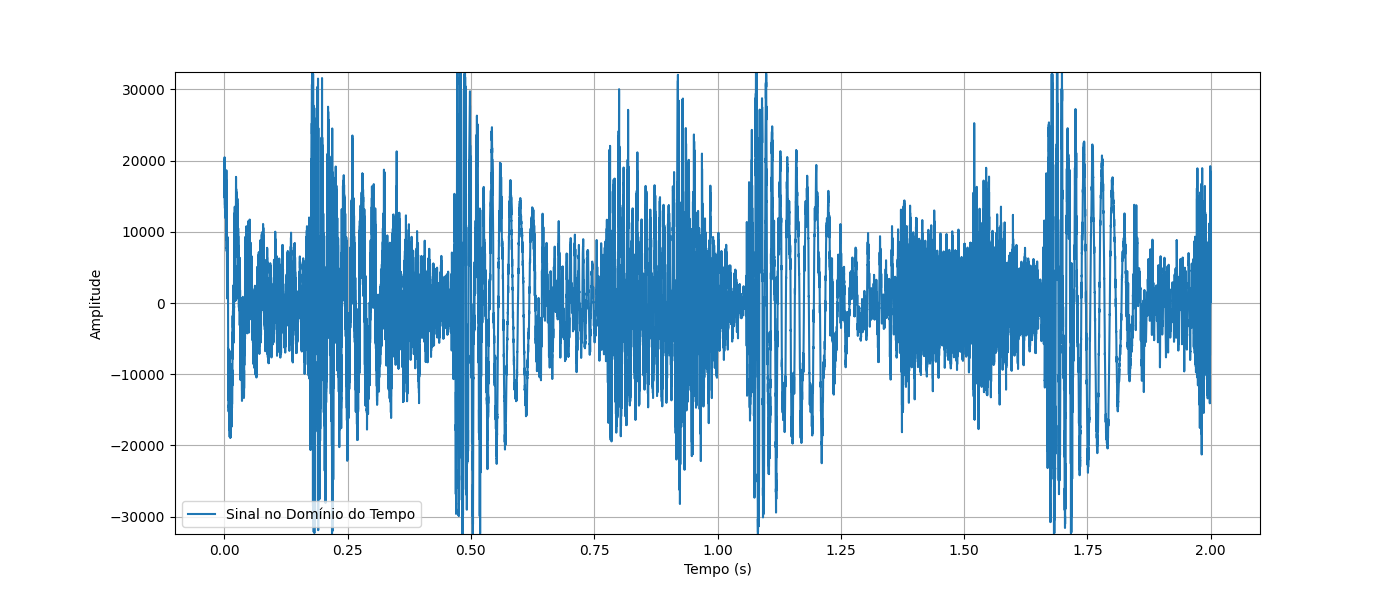
\includegraphics[width=0.8\textwidth]{figuras/fig40.png}
	\caption{música 1 no domínio do tempo sem filtragem}
	\label{fig40}
\end{figure}

Na Figura \ref{fig41}, a STFT dessa janela aponta a maior presença de elementos em baixa frequência. Da mesma forma como visto na Figura \ref{fig40}, percebe-se a variação de elementos de agudos conforme varia o andamento da música. 

\begin{figure}[h]
	\centering
    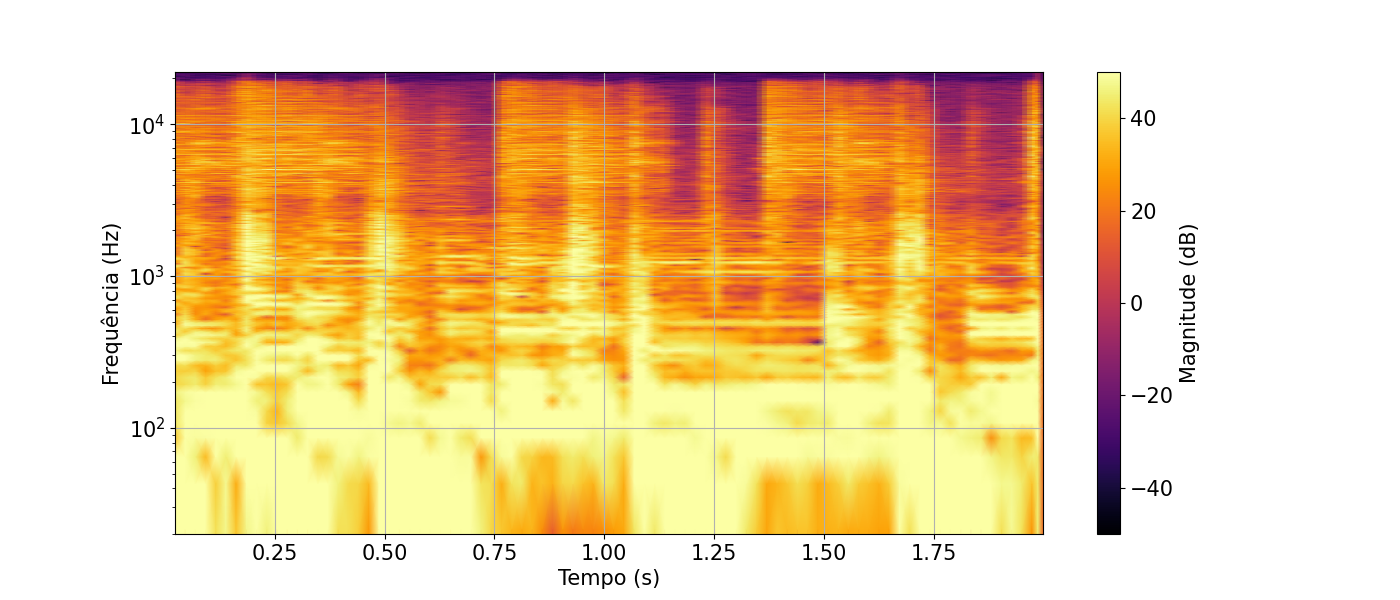
\includegraphics[width=0.8\textwidth]{figuras/fig41.png}
	\caption{música 1 no domínio da frequência sem filtragem}
	\label{fig41}
\end{figure}

Posteriormente, um filtro passa-altas de 20 Hz foi aplicado ao sinal. Na Figura \ref{fig24}, pouco se percebe a alteração do sinal.

\begin{figure}[h]
	\centering
    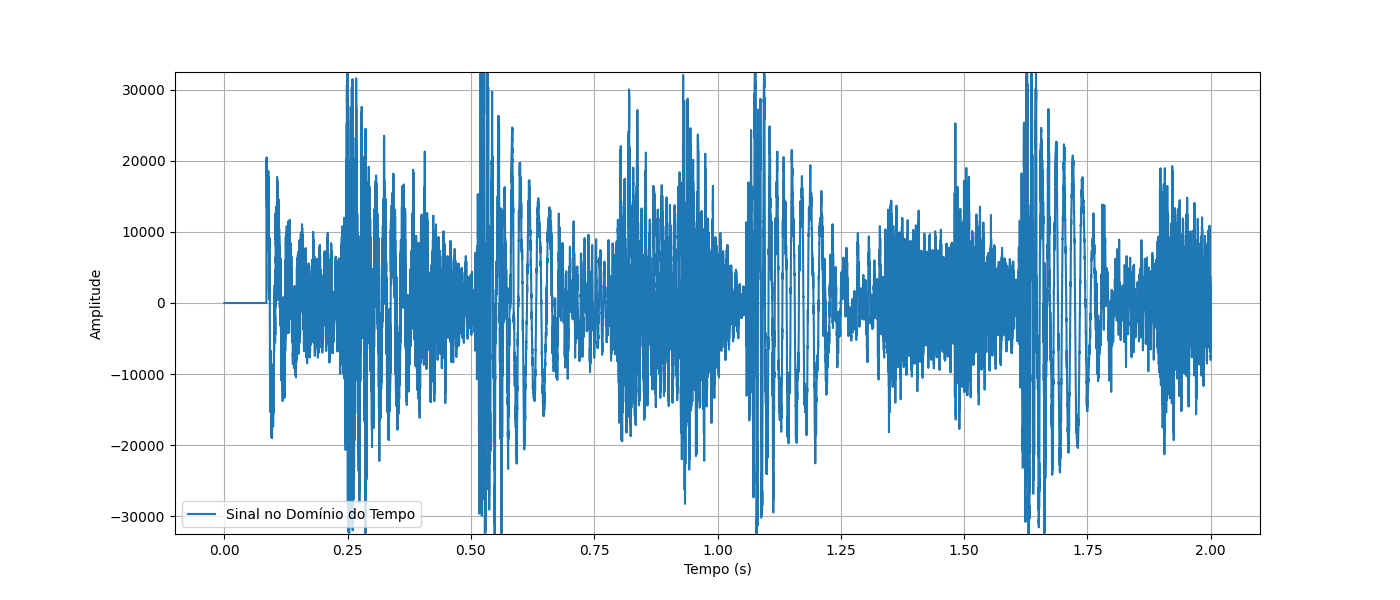
\includegraphics[width=0.8\textwidth]{figuras/fig24.png}
	\caption{música 1 no domínio do tempo com uma $f_c$ de 20 Hz}
	\label{fig24}
\end{figure}

O mesmo pode ser inferido ao se analisar a Figura \ref{fig25}, na qual não se percebe grandes alterações das componentes em frequência após a aplicação do filtro a uma frequência de corte de 20 Hz.

\begin{figure}[h]
	\centering
    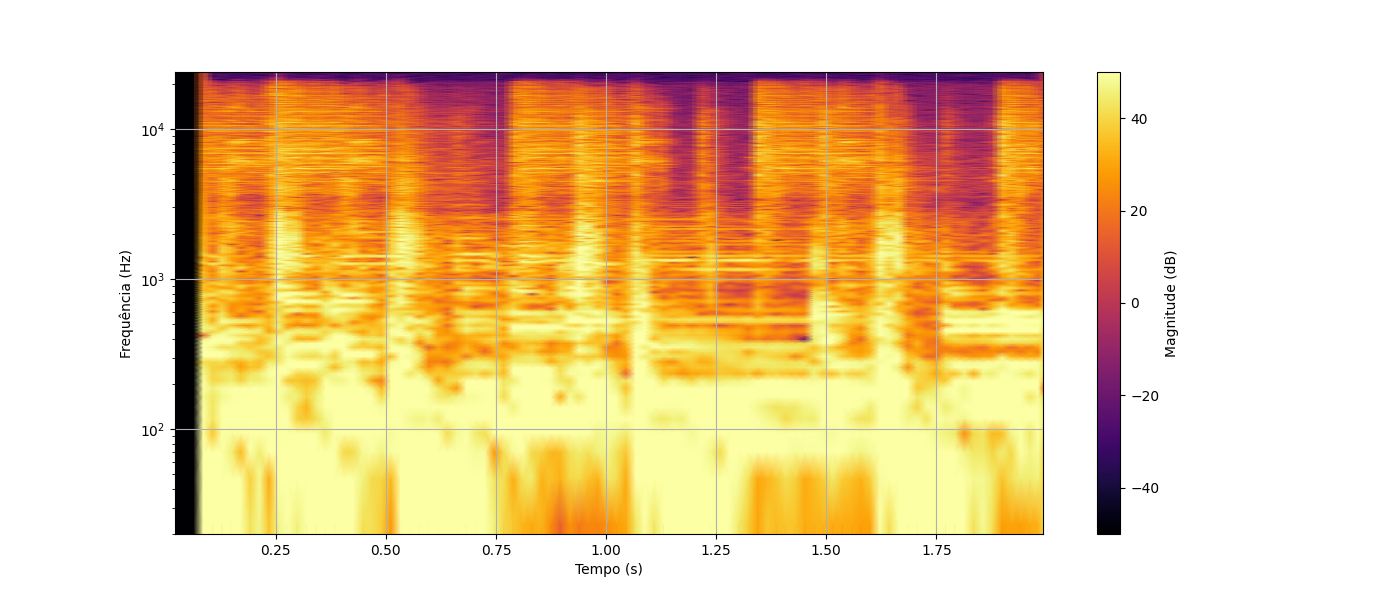
\includegraphics[width=0.8\textwidth]{figuras/fig25.png}
	\caption{música 1 no domínio da frequência com uma $f_c$ de 20 Hz}
	\label{fig25}
\end{figure}

Em \textit{mixers} convencionais, o botão correspondente às baixas frequências utiliza um controle de ganho na banda de 300 Hz. Dessa forma, deslocou-se o controle de frequência para que a frequência de corte se aproximasse de 300 Hz.

O resultado dessa filtragem pode ser visto nas Figuras \ref{fig28} e \ref{fig29}. Ao analisar a primeira figura, percebe-se a atenuação significativa dos sinais ao visualizar os valores máximo alcançados pela amplitude.

Além disso, percebe-se também a ausência de sinais de baixa frequência, presentes na forma de envelopes nos sinais anteriores. 

\begin{figure}[h]
	\centering
    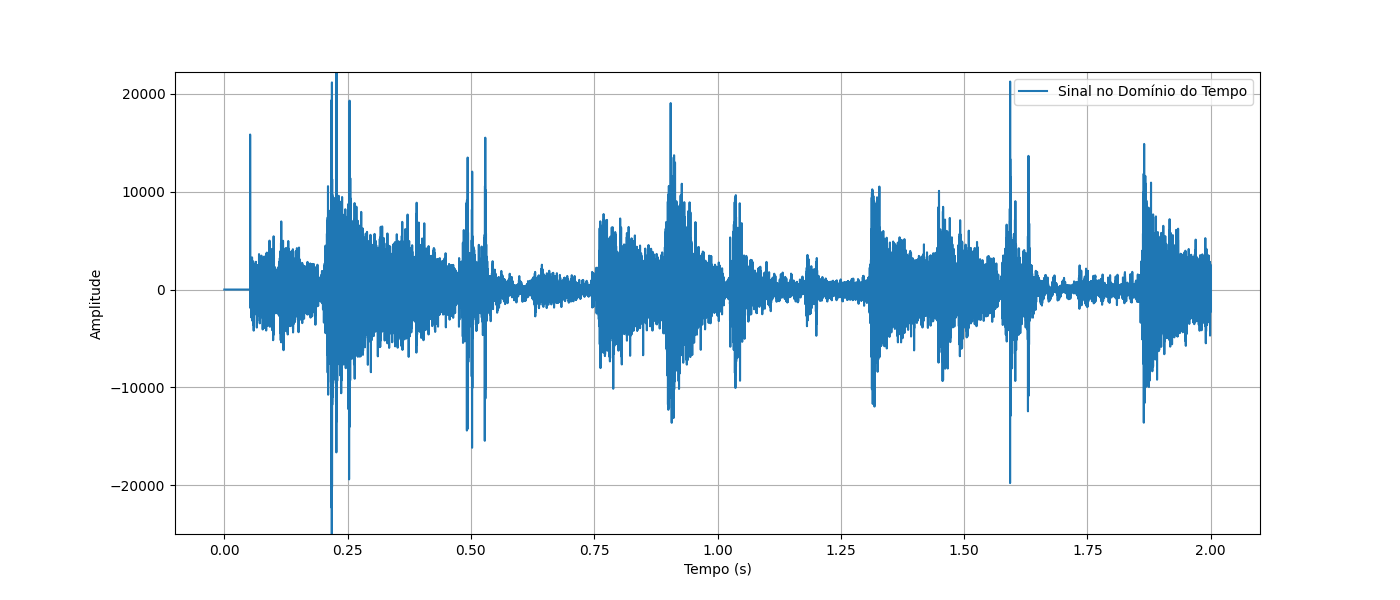
\includegraphics[width=\textwidth]{figuras/fig28.png}
	\caption{música 1 no domínio do tempo com uma $f_c$ de 300 Hz}
	\label{fig28}
\end{figure}

A atenuação dessa banda pode ser verificada na Figura \ref{fig29}, onde se percebe a atenuação dos sinais de baixa frequência de aproximadamente 30 dB.

\begin{figure}[h]
	\centering
    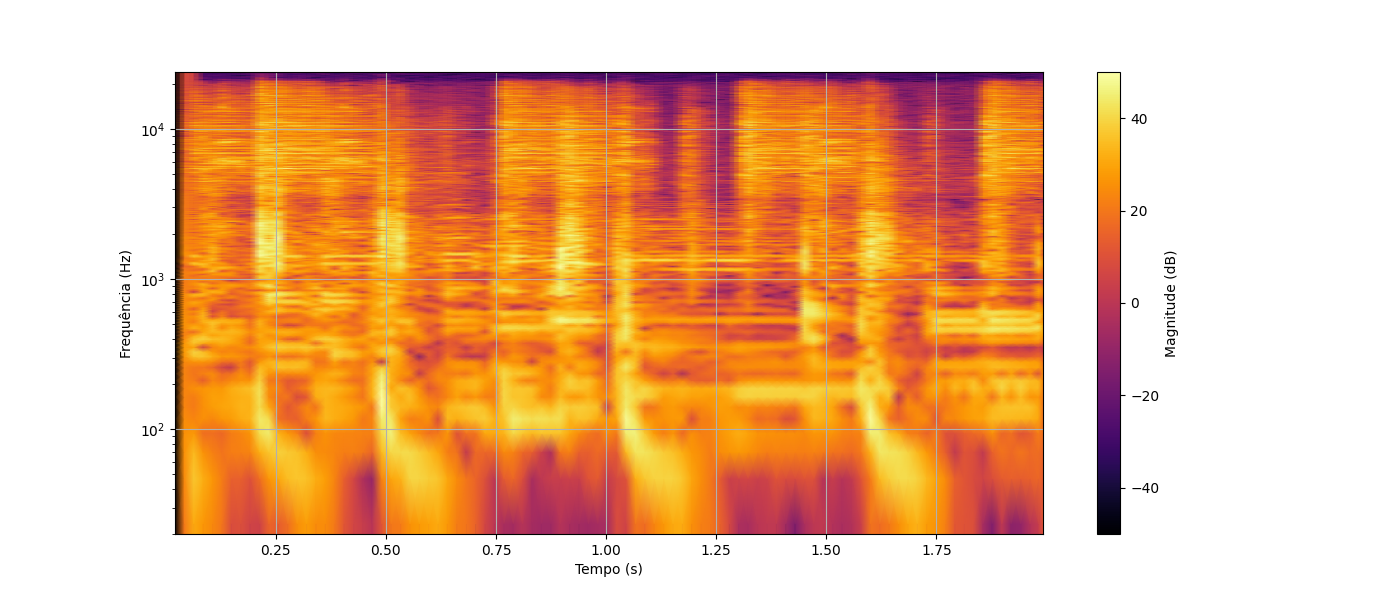
\includegraphics[width=0.8\textwidth]{figuras/fig29.png}
	\caption{música 1 no domínio da frequência com uma $f_c$ de 300 Hz}
	\label{fig29}
\end{figure}

A próxima frequência de corte utilizada foi de 4 kHz, que conforme infere o capítulo \ref{cha:fundamentacao}, é onde se encontram os elementos médios. Inicialmente, na Figura \ref{fig26} já se percebe a ateunação dos sinais em relação às filtragens anteriores.

\begin{figure}[h]
	\centering
    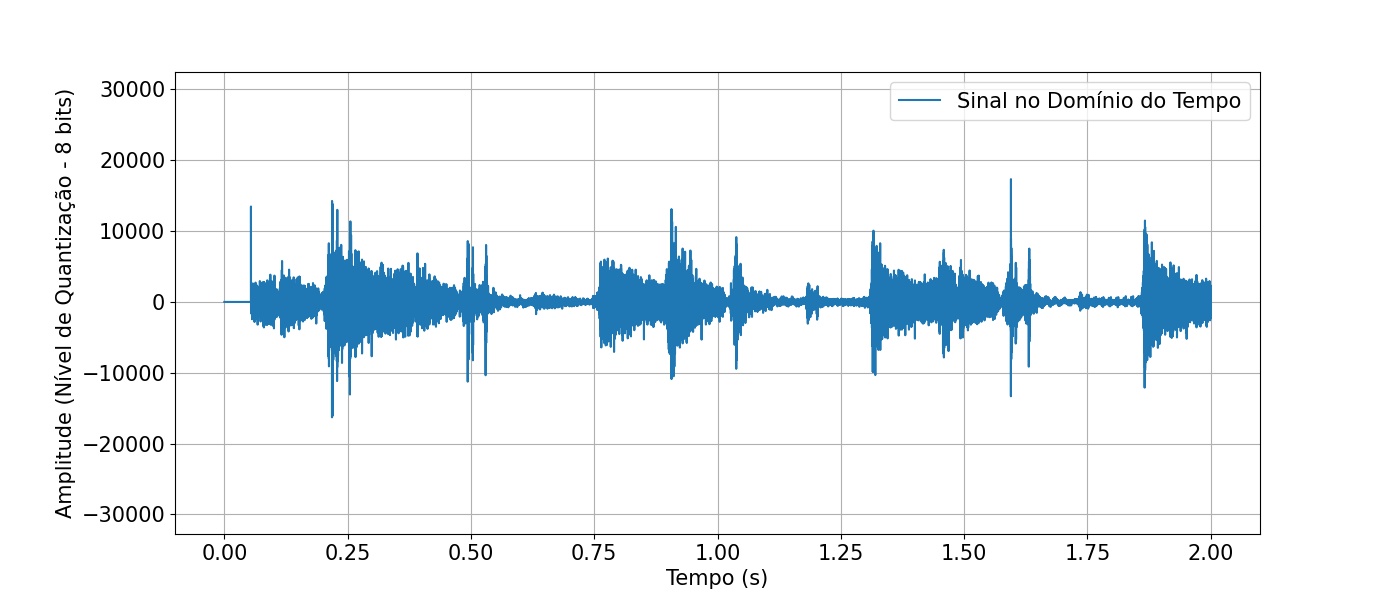
\includegraphics[width=0.8\textwidth]{figuras/fig26.png}
	\caption{música 1 no domínio do tempo com uma $f_c$ de 4 kHz}
	\label{fig26}
\end{figure}

Porém, na Figura \ref{fig27}, onde há a STFT, observa-se a atenuação das componentes referentes à presente banda de frequência. A queda foi bastante acentuada, encontrando-se componentes em 0 dB em determinados pontos.

\begin{figure}[h]
	\centering
    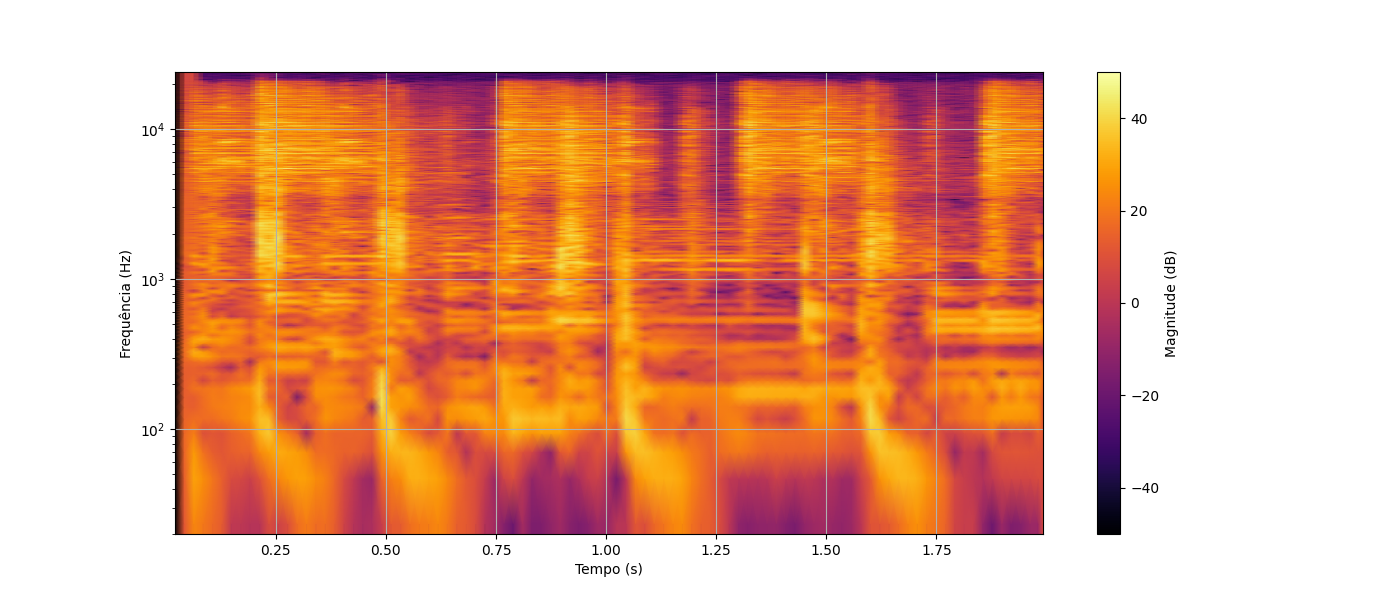
\includegraphics[width=0.8\textwidth]{figuras/fig27.png}
	\caption{música 1 no domínio da frequência com uma $f_c$ de 4 kHz}
	\label{fig27}
\end{figure}

Para a música \cite{track01}, uma última análise foi realizada considerando que a filtragem foi realizada em toda banda. Dessa forma, utilizou-se uma frequência de corte de 24 kHz, de forma que os elementos restantes, tidos como agudos ou brilhos, fossem atenuados. Assim, verifica-se na Figura \ref{fig30} uma atenuação de amplitudes de sinais quando comparados com as filtragens anteriores.

\begin{figure}[h]
	\centering
    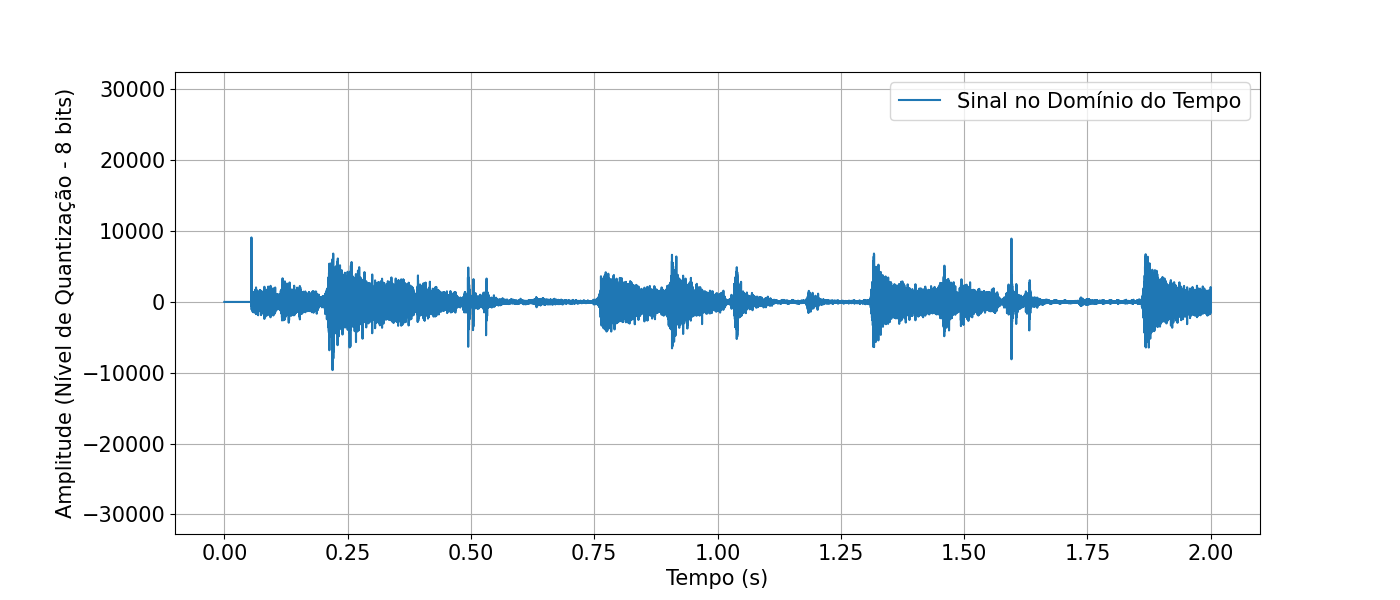
\includegraphics[width=0.8\textwidth]{figuras/fig30.png}
	\caption{música 1 no domínio do tempo com uma $f_c$ de 22 kHz}
	\label{fig30}
\end{figure}

Além disso, na Figura \ref{fig31}, percebe uma atenuação da banda correspondente, contendo elementos de 10 dB a -40 dB. E ao comparado com a STFT da filtragem anterior, percebe-se uma atenuação generalizada do sinal.

\begin{figure}[h]
	\centering
    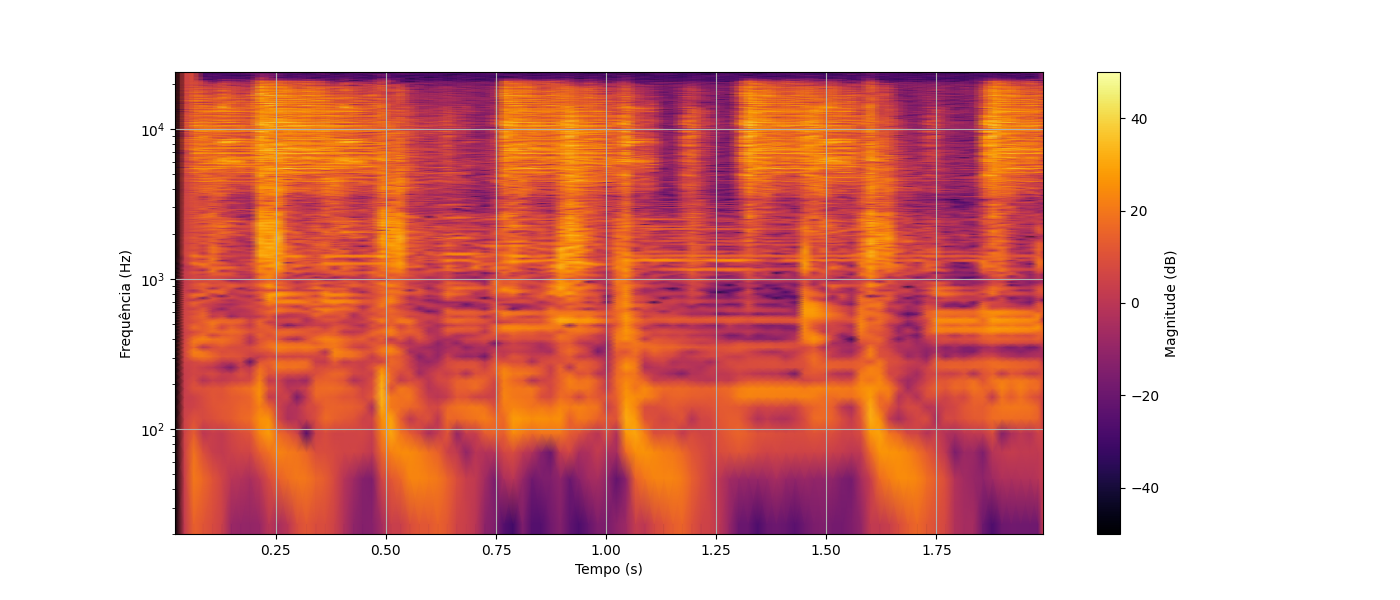
\includegraphics[width=0.8\textwidth]{figuras/fig31.png}
	\caption{música 1 no domínio da frequência com uma $f_c$ de 22 kHz}
	\label{fig31}
\end{figure}

A mesma análise realizada na Música \cite{track01} foi realizada a Música \cite{track02}, de forma que os resultados no domínio do tempo e da frequência, utilizando a STFT, foram obtidos. O comportamento obtido foi semelhante ao obtido na análise da música \cite{track01}.

Deve-se atentar que conforme o botão avança na frequência de corte, a frequência de corte do filtro do canal 1 aumenta, de forma que as componentes são atenuadas começando pelas menores frequências e finalizando na maior frequência, enquanto para o canal 2, a frequência de corte começa sendo a máxima e termina sendo a mínima, de forma que as figuras mostrem as ampliações das componentes de frequência do sinal da Música \cite{track02}.

\section{Resultados de Efeitos}

Os efeitos são operados de forma que a frequência central determina qual será o volume do efeito e um botão de duas posições seleciona qual efeito será utilizado. Assim, testes dessas operações foram realizados. 

Primeiramente, simulou-se o volume do efeito em relação a posição do botão central. Posteriormente, simulações variando os parâmetros dos efeitos foram realizadas. 

\subsection{Automação de Efeitos}

Para validar o controle automático do volume, isolou-se a saída dos efeitos e variações de frequências, que dão origens a diferentes volumes de efeitos, a fim de se obter sinais no domínio do tempo, conforme as figuras abaixo. 

Na Figura \ref{fig66}, a frequência central utilizada foi a mínima. Dessa forma, conforme a função da Figura \ref{fig49}, o volume esperado seria nulo. Dessa forma, o sinal esperado também seria constante nulo, conforme o que foi obtido.

\begin{figure}[h]
	\centering
    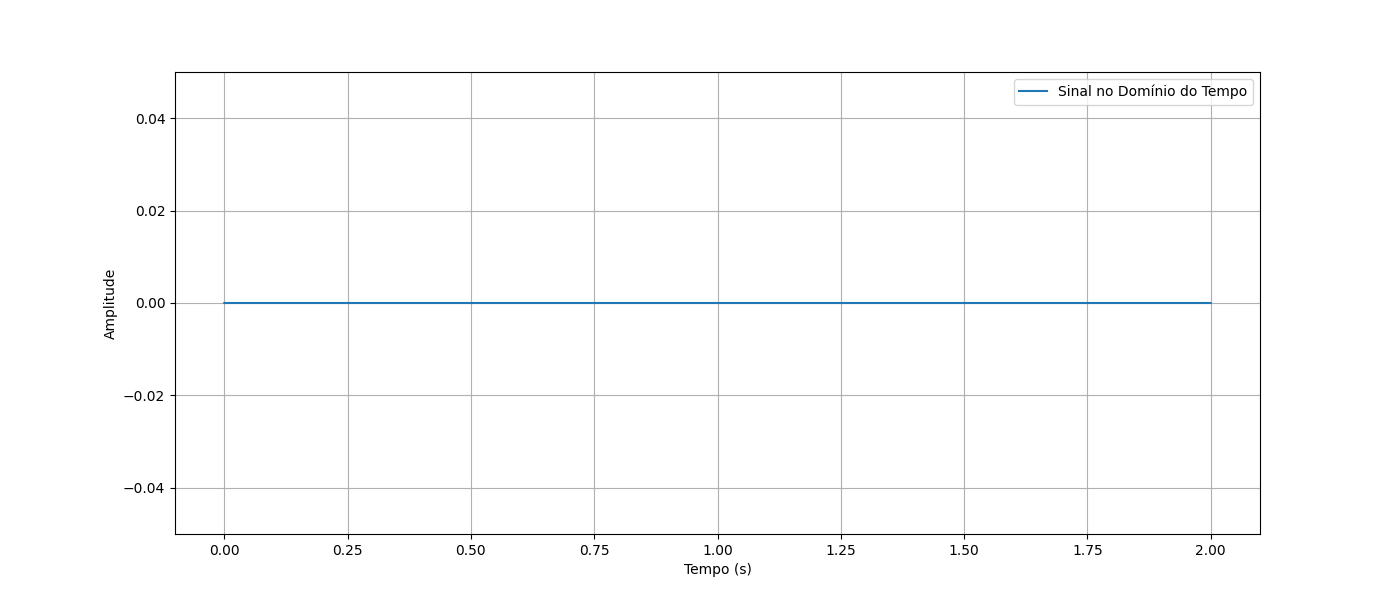
\includegraphics[width=0.8\textwidth]{figuras/fig66.png}
	\caption{canal de efeito \textit{reverb} isolado com música 1 a um volume nulo}
	\label{fig66}
\end{figure}

Posteriormente, variou-se a posição do botão central para que se alcancasse a frequência de 9454 Hz, que gera um volume de 0.3312. Assim, conforme a Figura \ref{fig67}, obteve-se um sinal similar à música \cite{track01} com determinada amplitude. 
 
\begin{figure}[h]
	\centering
    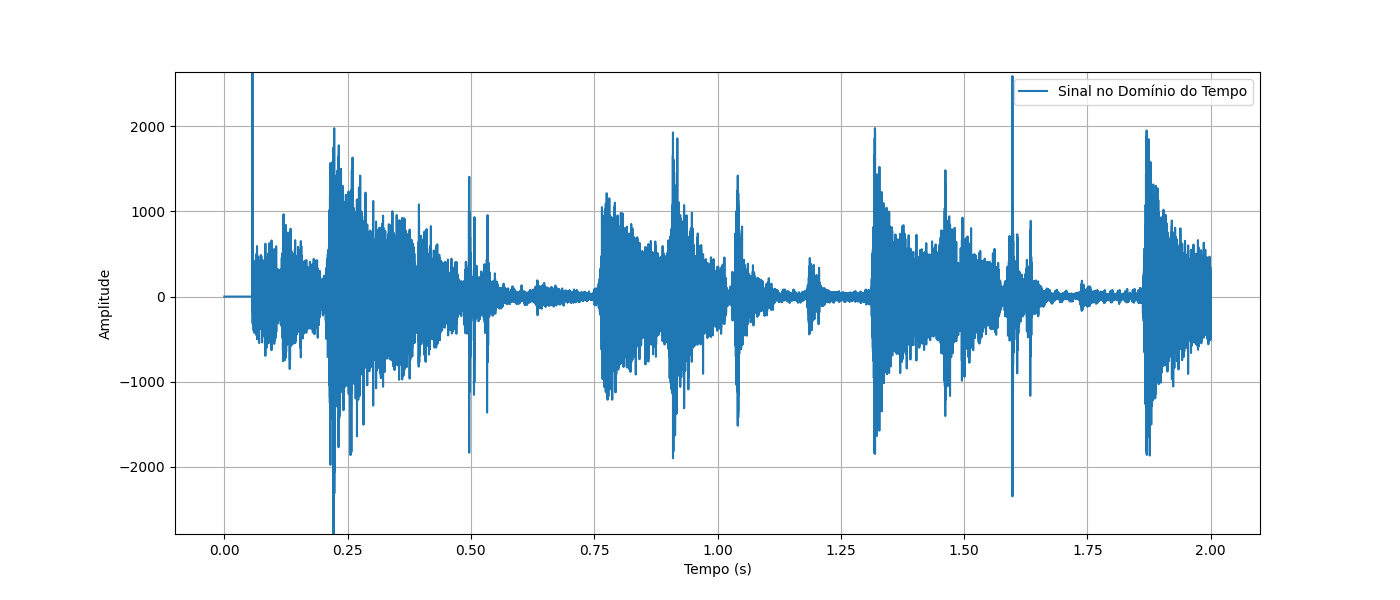
\includegraphics[width=0.8\textwidth]{figuras/fig67.png}
	\caption{canal de efeito \textit{reverb} isolado com música 1 a um volume de 0.3312}
	\label{fig67}
\end{figure}

Variou-se a posição do botão central a fim de visualizar a variação do volume do efeito. Dessa forma, a próxima frequência utilizada foi de 9875 Hz. Obteve-se um volume maior, como se pode visualizar na Figura \ref{fig68}.

\begin{figure}[h]
	\centering
    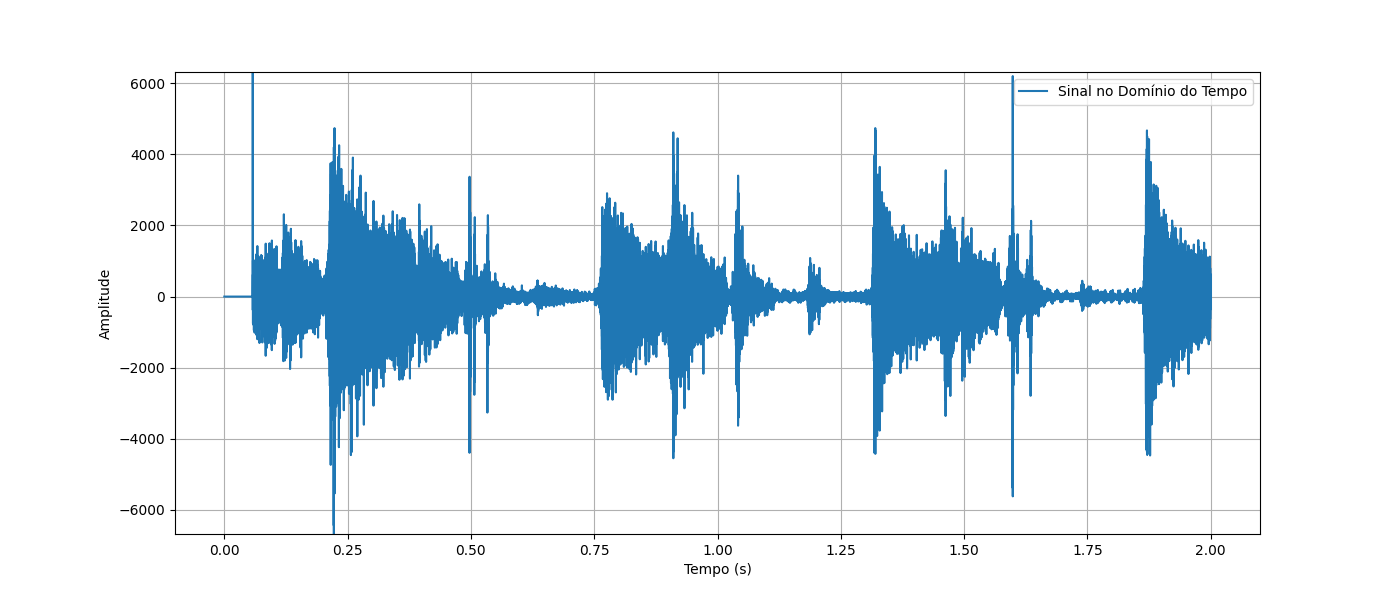
\includegraphics[width=0.8\textwidth]{figuras/fig68.png}
	\caption{canal de efeito \textit{reverb} isolado com música 1 a um volume de 0.6625}
	\label{fig68}
\end{figure}

Para validar completamente a automação do volume, posicionou-se o botão central na frequência de 11025 Hz, que gera o volume máximo unitário. Assim, pôde-se observar a ampliação do volume em função da variação da frequência de forma que se valide a automação do volume.

\begin{figure}[h]
	\centering
    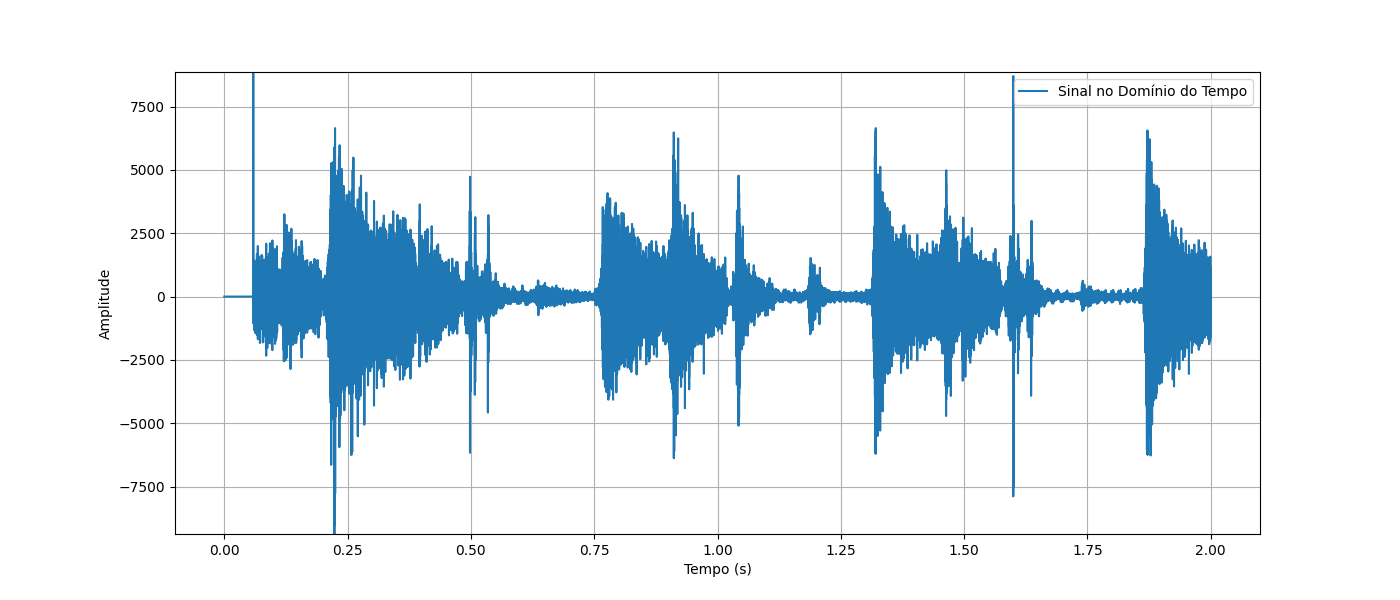
\includegraphics[width=0.8\textwidth]{figuras/fig69.png}
	\caption{canal de efeito \textit{reverb} isolado com música 1 a um volume igual a 1.0}
	\label{fig69}
\end{figure}

\subsection{\textit{Reverb}}

Para a validação do controle de presença de efeitos, o botão central foi posicionado de forma que a frequência selecionada conferisse o volume máximo para efeitos. Em seguida, alterou-se a posição do botão de presença de efeito a fim de visualizar a variação dos parâmetros de efeito. No caso de \textit{reverb}, ao se variar o parâmetro, a quantidade de dB presente após 1s é configurada conforme o botão de parâmetro. 

Nas figuras a seguir, pode-se observar Figuras que representam o sinal no domínio do tempo nos quais é possível observar a variação desse parâmetro. O intervalo de dB proposto nesse sistema varia de 0 a 1000 dB.

Na Figura \ref{fig70}, a posição do botão de quantidade de efeito foi a inicial, ou seja, a quantidade de dB presente após 1s é nula. Dessa forma, a forma de onda esperada seria também nula, conforme o que foi obtida.


\begin{figure}[h]
	\centering
    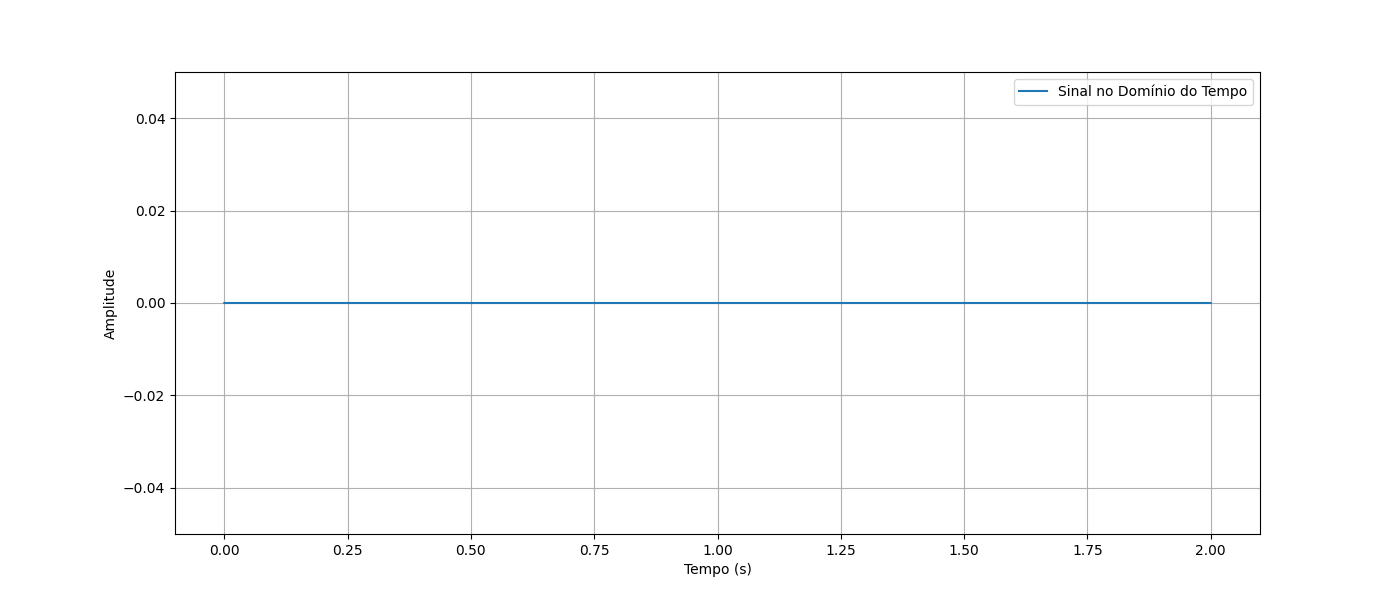
\includegraphics[width=0.8\textwidth]{figuras/fig70.png}
	\caption{\textit{reverb} com 0 dB após 1s}
	\label{fig70}
\end{figure}

Posteriormente, posicionou-se o botão de parâmetro de efeito de forma que 25 dB permanecesse após 1s da amostra atual da música. Assim, conforme a Figura \ref{fig71}, pôde-se observar a repetição de trechos da música. 

\begin{figure}[h]
	\centering
    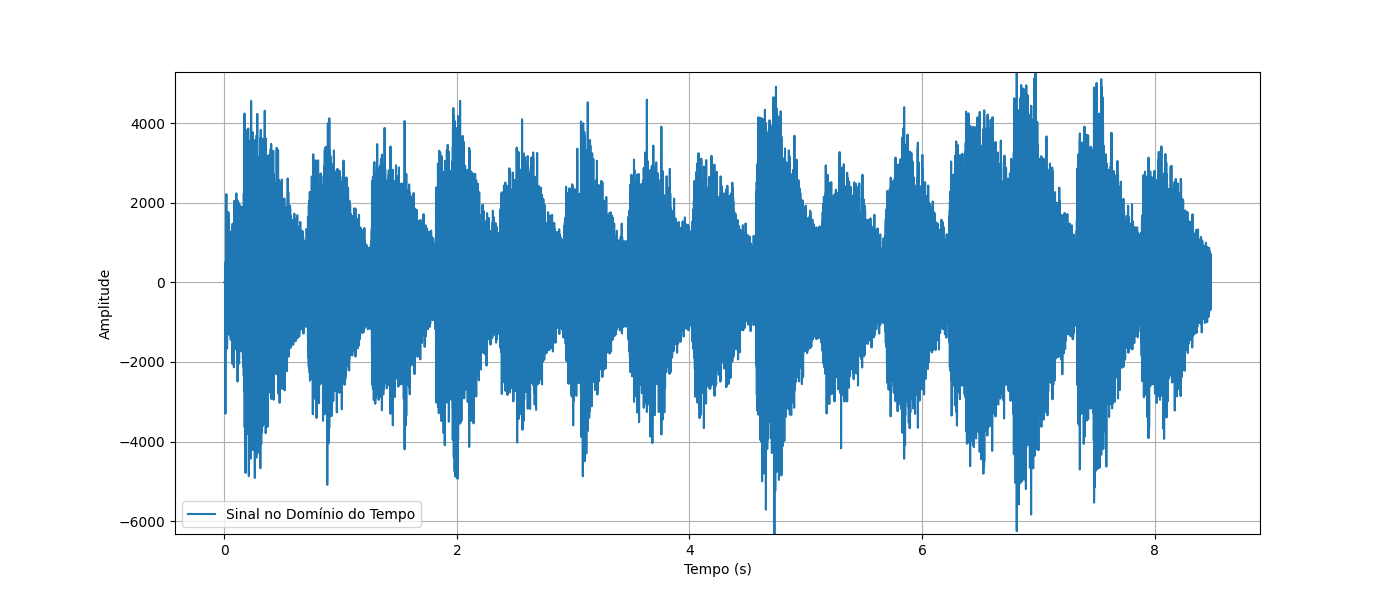
\includegraphics[width=0.8\textwidth]{figuras/fig71.png}
	\caption{\textit{reverb} com 25 dB após 1s}
	\label{fig71}
\end{figure}

Porém, conforme o ganho da música é aumentado, mais se percebe o efeito de um \textit{reverb}. Na Figura \ref{fig72}, pôde-se observar maior presença desse efeito visto que o sinal obtido possuiu uma amplitude maior ao longo do tempo.

\begin{figure}[h]
	\centering
    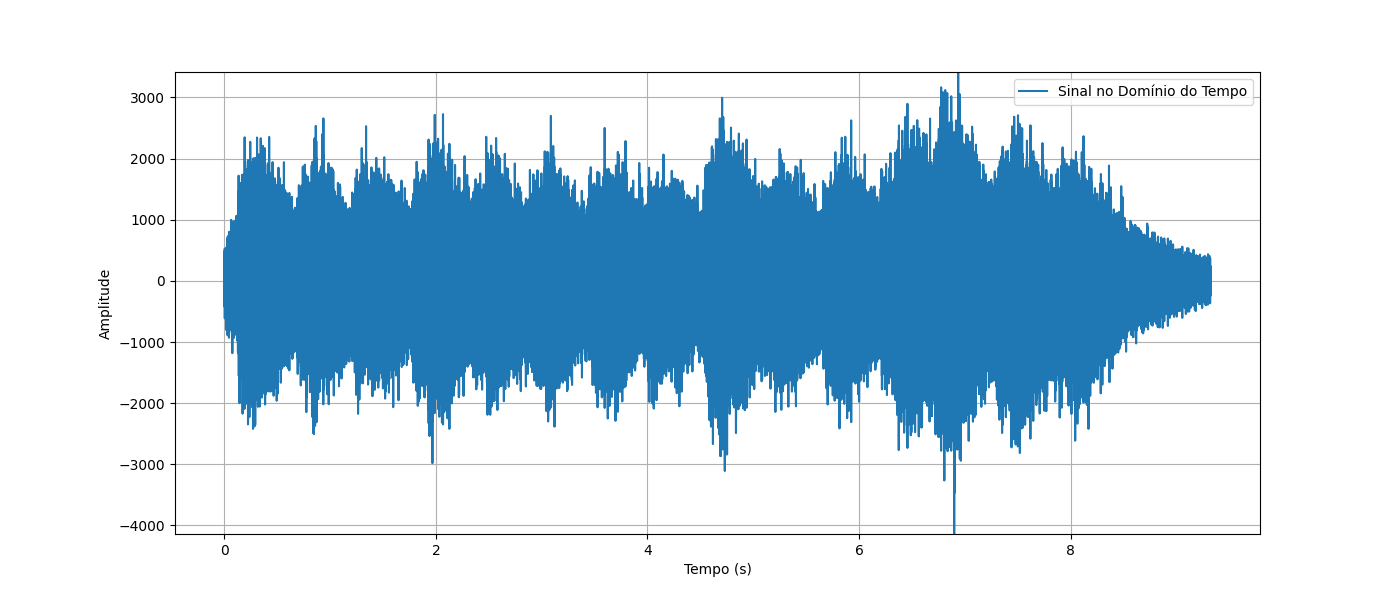
\includegraphics[width=0.8\textwidth]{figuras/fig72.png}
	\caption{\textit{reverb} com 50 dB após 1s}
	\label{fig72}
\end{figure}

O mesmo efeito pôde ser observado ao se configurar 100 dB de ganho após 1s na Figura \ref{fig73}, visto que essa imagem representa um som com pouca definição, o que infere que maior quantidade de som permaneceu de forma que a nitidez da música se perdeu.

\begin{figure}[h]
	\centering
    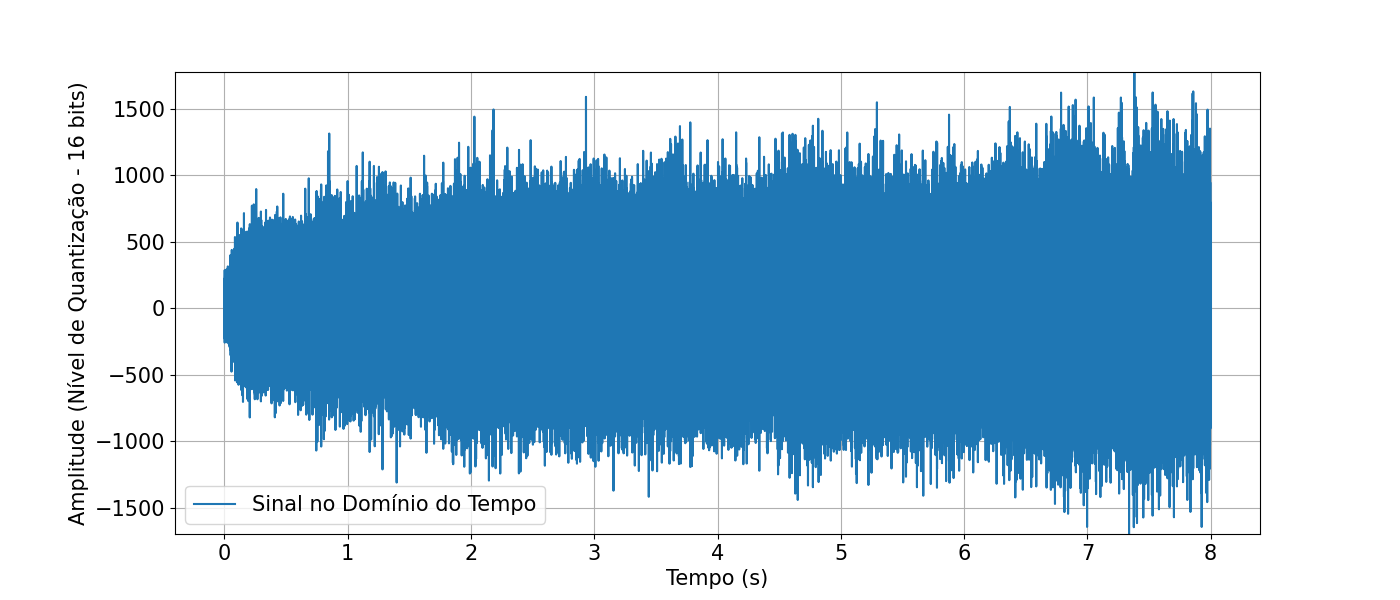
\includegraphics[width=0.8\textwidth]{figuras/fig73.png}
	\caption{\textit{reverb} com 100 dB após 1s}
	\label{fig73}
\end{figure}

\subsection{\textit{Delay}}

No caso do efeito de \textit{delay}, as amostras são repetidas a determinado tempo depois que os sinais são lidos. Assim, as figuras a seguir mostram a repetição desse sinal. Percebe-se que não há alteração do ganho do sinal nem do período em que o sinal permanece. Assim, os sinais simplesmente são repetidos.

Na Figura \ref{fig74}, um \textit{delay} de 0 ms foi configurado. Assim, uma cópia do sinal foi obtida porém concomitante conforme o sinal é lido. 

\begin{figure}[h]
	\centering
    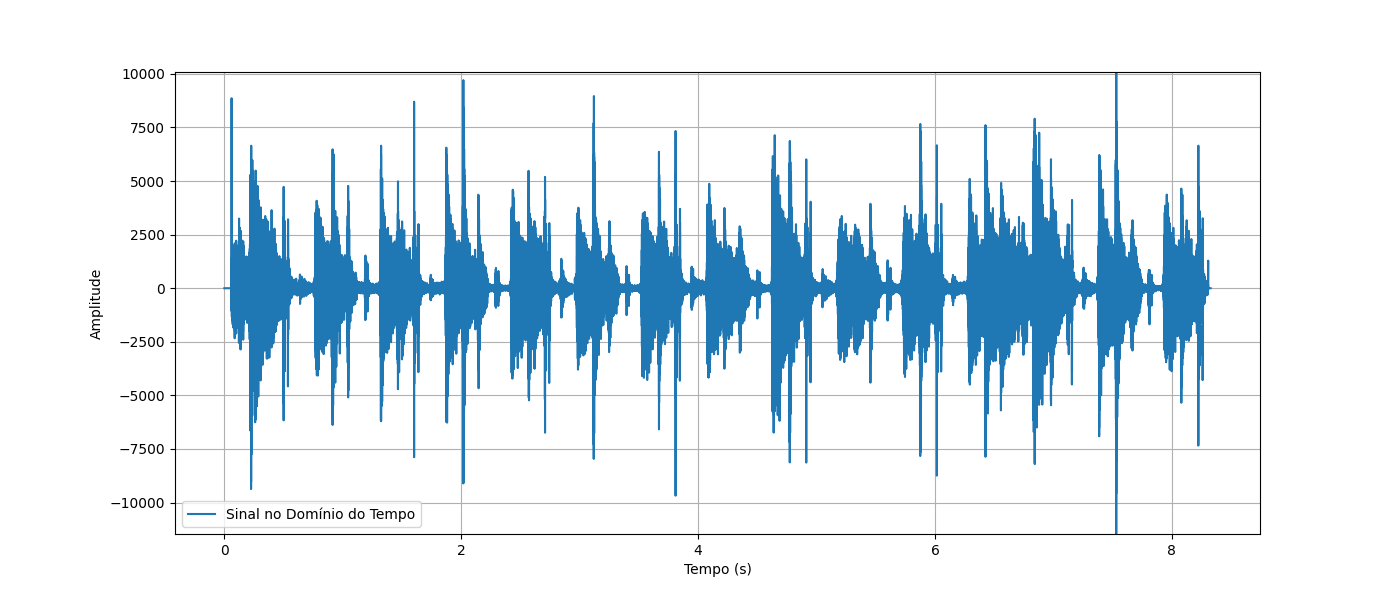
\includegraphics[width=0.8\textwidth]{figuras/fig74.png}
	\caption{\textit{delay} de 0 ms}
	\label{fig74}
\end{figure}


Na Figura \ref{fig74}, um \textit{delay} de 250 ms foi configurado. Assim, uma cópia do sinal foi obtida e reproduzida conforme o tempo configurado.

\begin{figure}[h]
	\centering
    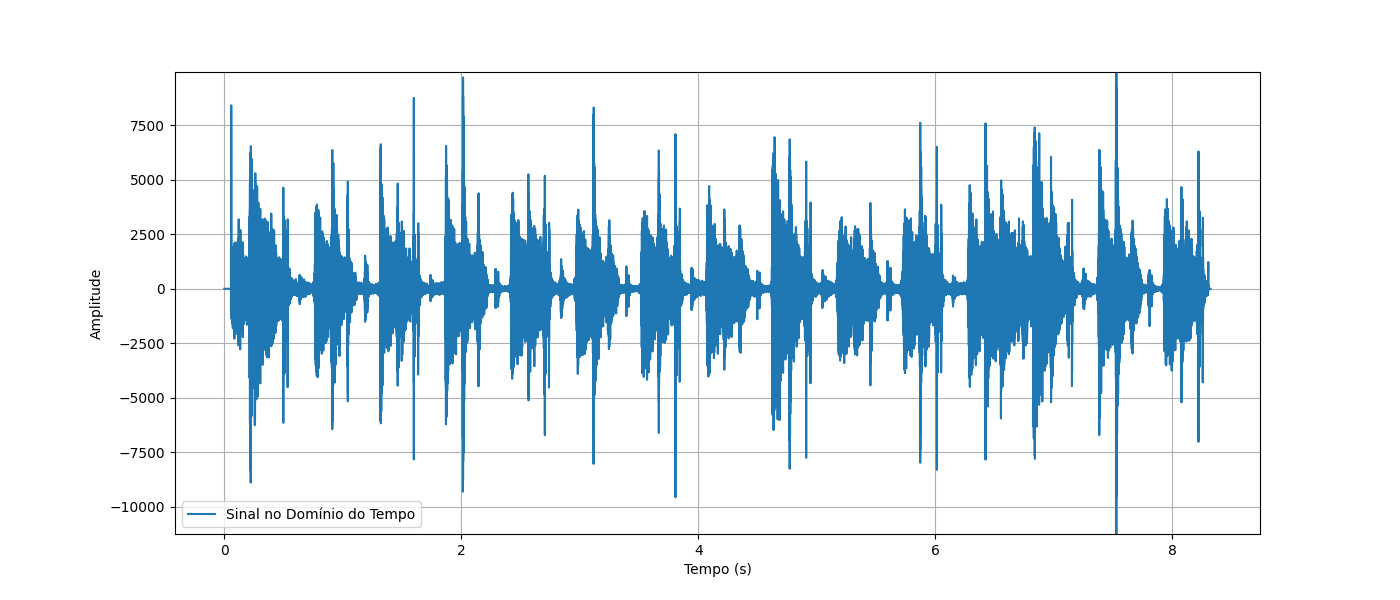
\includegraphics[width=0.8\textwidth]{figuras/fig75.png}
	\caption{\textit{delay} de 250 ms}
	\label{fig75}
\end{figure}

Na Figura \ref{fig74}, um \textit{delay} de 500 ms foi configurado. Assim, uma cópia do sinal foi obtida e reproduzida conforme o tempo configurado.

\begin{figure}[h]
	\centering
    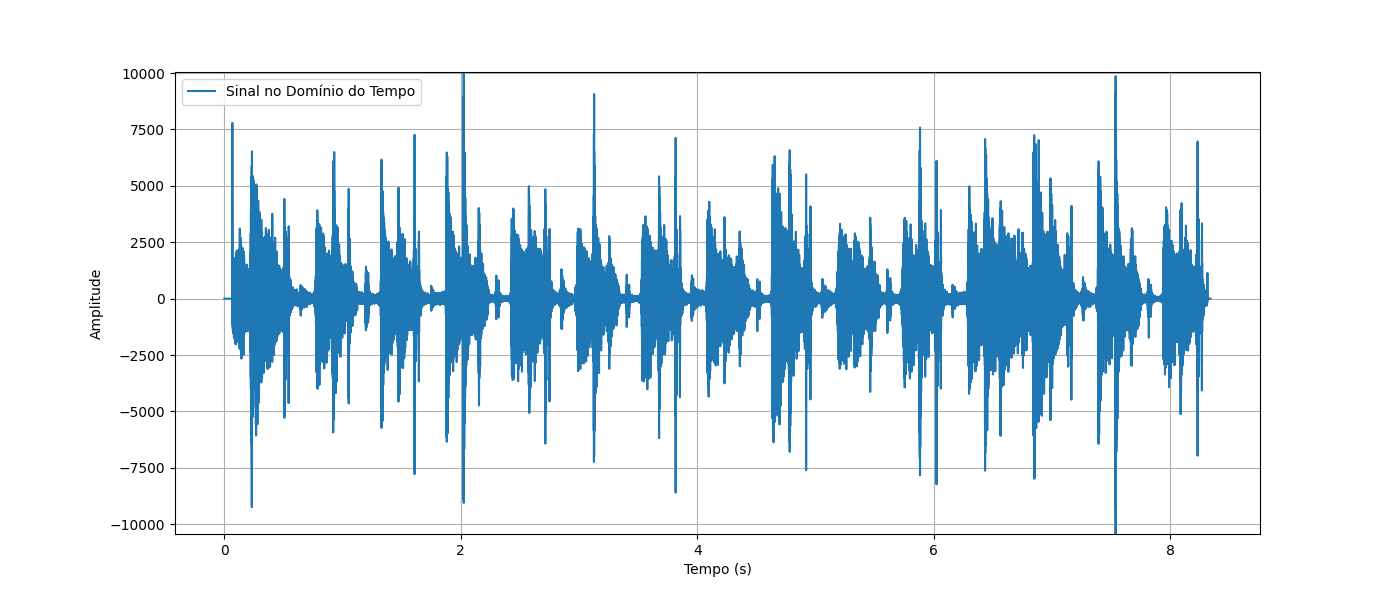
\includegraphics[width=0.8\textwidth]{figuras/fig76.png}
	\caption{\textit{rdelay} de 500 ms}
	\label{fig76}
\end{figure}

Na Figura \ref{fig74}, um \textit{delay} de 1000 ms foi configurado. Assim, uma cópia do sinal foi obtida e reproduzida conforme o tempo configurado.

\begin{figure}[h]
	\centering
    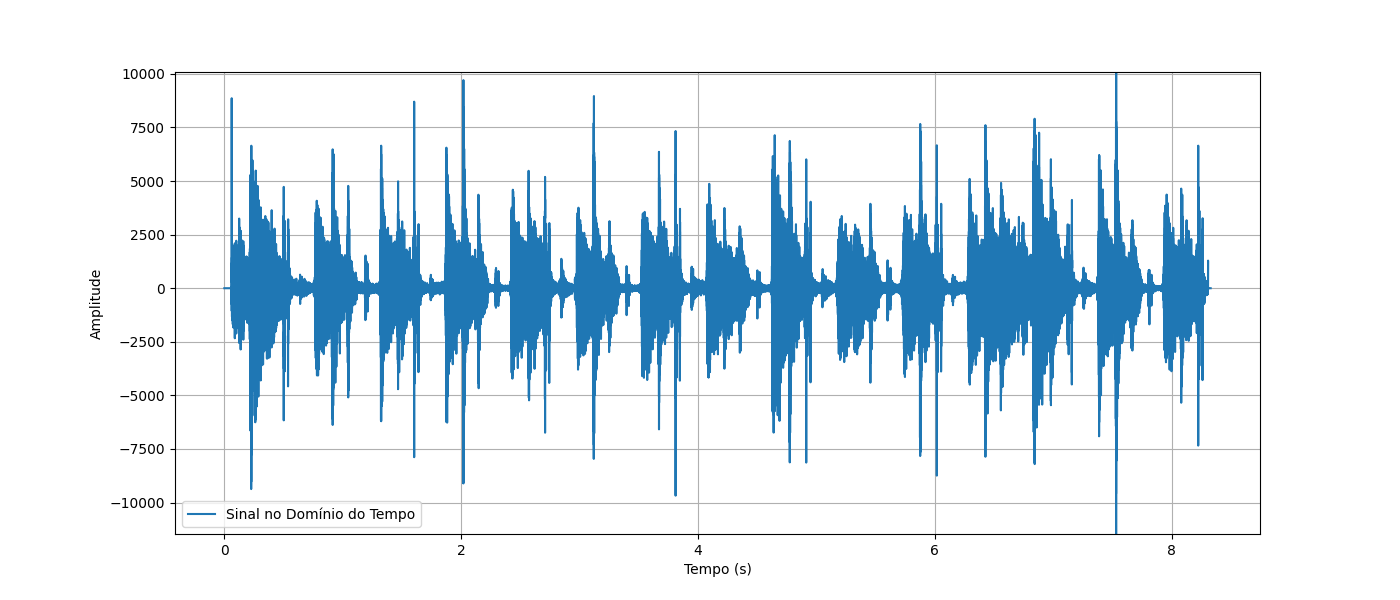
\includegraphics[width=0.8\textwidth]{figuras/fig77.png}
	\caption{\textit{delay} de 1000 ms}
	\label{fig77}
\end{figure}
